%       %======================================================================
%       %  SubSection
%       %======================================================================
\subsection{写像とは}
    集合についてはこのくらいにして,次に \textbf{写像} という概念を考えて
    いこう.集合を2つもってきて,それらをA,Bとしよう.集合Aの各要素に対し
    て,集合Bの要素を対応させる.この対応の方法は様々だが, これを $f$
     という記号を用いて,
        \begin{equation*}
            f\,:\,A \longmapsto  B
        \end{equation*}
    と表現する.この $f$ のことを写像という.記号の意味は,写像 $f$ によっ
    て,集合Aの要素を集合Bの要素に対応させるということである.対応のさせ方
    は大きく分けて3つがある.それは,
    \textbf{全射},\textbf{単射},\textbf{全単射} である.

    全射とは,例えば,もとの集合Aの要素を別の集合Bの要素に対応させるときに,
    Aの要素に漏れが1つもなくBの全ての要素に対応していることである.ここで,
    Aの複数の要素がBの1つの要素に対応していてもかまわない.とにかく,全射
    とはもとの集合から漏れる要素が1つもなく,別の集合の要素に対応している
    状況のことをいう.但し注意しておくことは,集合Aの要素1つから集合Bの複
    数の要素には    対応していないことである.簡単にいえば,集合Aの要素を1
    つもってきたとき,それに対応するB要素がただ1つ定まっていることである.

        \begin{figure}[hbt]
            \begin{center}
                \includegraphicsdefault{zensha1.pdf}
                \caption{全射のイメージ}
                \label{fig:zensha1}
            \end{center}
        \end{figure}

    よく知っている例では,2次関数 $f(x)=x^{2}$ がある.これは写像 $f$ を
    使って表現すると次のようになる.
        \begin{equation*}
            f\,:\,x \longmapsto  x^{2}
        \end{equation*}
    $x$ が1つ定まると,$x^{2}$ の値は必ず1つ定まる.
    例えば $x=2$ のとき,$x^{2}=4$ である
        \footnote{
            ここが混乱しやすい部分だが,$x=-2$ の時も $x^{2}=4$ である.
            確かに,$x=2$ と $x=-2$ の場合の両方で,写像 $f$ に
            よって同じ値( $x^{2}=4$ )に対応させられているが,これは全く問
            題はない.ここで考えているのは $x$ から $x^{2}$ を対応させるよ
            うな写像 $f$ であって,$x^{2}$ から $x$ に対応させる写像ではな
            いからだ.
        }.

    次に \textbf{単射} について考える.単射であるとは漏れはあるが,重複はないという
    ことを意味する.もとの集合Aの全ての要素は別の集合Bの要素に対応している
    という約束はあるが,集合Bの全てに対応している必要はない.つまり,集合B
    側には要素の漏れがあってもよい.単射で大事なのは,重複した対応がないと
    いうことである.
        \begin{figure}[hbt]
            \begin{center}
                \includegraphicsdefault{tansha1.pdf}
                \caption{単射のイメージ}
                \label{fig:tansha1}
            \end{center}
        \end{figure}

    単射の例を考えれば,自然数を2倍して偶数にするという関数を上げられる.
    つまり,$f(x)=2x$ である.写像の表記をすれば,
        \begin{equation*}
            f\,:\,\bN \longmapsto
            \bN\;,\quad f\,:\,x \longmapsto  2x
        \end{equation*}
    である.但し,ここでの $x$ は自然数に限っている.はじめに書いた
     $f\,:\,\bN \longmapsto \bN$ は
    自然数から自然数への写像であることを示し($\bN$ は自然
    数を表現する),その後に書いた $f\,:\,x \longmapsto  2x$ は自然数を2倍
    して偶数を求めるという写像を意味している.そうすれば確かに,$x$ はすべ
    て $2x$ に写せる.$2x$ は自然数の一部であり,全体ではない
        \footnote{
            しかし,自然数の濃度と偶数の濃度は同じである.“濃度”について
            は,集合論などの教科書を参照.濃度とは,簡単にいえば,要素の個
            数が無限大個であるときの,集合の“大きさ”を示すものである.
        }.

%       %======================================================================
%       %  SubSection
%       %======================================================================
\subsection{関数}
    次に,関数について確認するが,これは簡単だ.実数から実数へ
    の写像を,慣習に従って,\textbf{関数} という.これだけである.高校の時
    には,「変数 $x$ が1つ定まったとき,それに伴って,$f(x)$ も1つに定まる
    ならば,$f(x)$ は$x$ の関数であるという」と習ったと思う.これは正しい.
    しかし,写像という概念を導入すると,数学の世界がもっと広くなる.なので,
    ここで写像という概念の紹介をしたかった.写像とはとても抽象的なものであ
    り,捉えるのが難しい.しかし,あえて感覚的に説明しようとすれば,写像と
    はある集合の要素を,何らかの変換を用いて,別の集合の要素に対応させるも
    のであるといえよう
        \footnote{
            この説明はどのくらい妥当かどうか不安.
        }.

%       %======================================================================
%       %  SubSection
%       %======================================================================
\subsection{関数のイメージ}
    関数のイメージとして,よく例に挙がるのは,“自動販売機”
    である
        \footnote{
            以降,自動販売機のことを“自販機”と略記する.
        }
    自販機を関数としてみる
    とき,それは,入力1つに対して,出力が1つであるという特徴
    を指している.入力とは,ほしい商品に対応したボタンを
    押すことであり,出力はそのほしい商品が取り出し口に
    現れることである.これは,関数のイメージによく合う.
    関数とは,
        \begin{equation*}
            \mbox{1つの入力に対して,1つの出力が対応する}
        \end{equation*}
    という性質をもつものである.

    数学ではよく関数を $f(x)$ のような記号で表現される.
    初めてこの記号をみると,面を食らってしまう.
    中学校で初めて習う一次関数は,$y=ax+b$ のように
    記述していたし,2次関数だって,$y=ax^{2}+bx+c$ と
    書かれた.この時に,$y$ は $x$ の一次関数だとか,
    2次関数だとかというように覚えさせられる.

    なぜ $f(x)$ のような書き方をするのか.
    それは,関数という概念を,一般化して考えたい
    からである.関数には,一次関数や2次関数
    に限らず,もっと高次元の $n$ 次関数とか,
    指数関数,三角関数とかいろいろ考えられる.
    これらの関数を,どれか1つに特定することなく,
    関数全てを対象にして考えたいときには,
    関数の具体的な形を与えるわけにはいかない.
    しかし,関数という以上,入力と出力を表現すべきだ.
    入力に対応するのが,記号 $f(x)$ の括弧の中の変数 $x$ で,
    出力は $f(x)$ そのもので表現される.
    入力とにそれに対応する出力は分かっているが,
    その具体的な形はわからないときに
        \footnote{
            もしくは,形を特定したくないとき.
        },
    $f(x)$ という記号を使うのである.こうすれば,
    関数一般について記述できるのである.
        \begin{equation*}
            \mbox{入力}  x \mbox{に対して,} f  \mbox{という操作を施して,}  f(x) \mbox{として出力する}
        \end{equation*}
    ということをこの記号は表現する.入力と操作方法が
    分かれば,出力も分かる.だから,入力と
    操作方法を象徴するような記号で関数を表せる.

    その内部の構造は知らなくてもよい.それは本当か.もう一度,
    自販機の例を考える.入力は,ほしい商品に対応するボタン
    を一回押すこと.出力は,ほしい商品が取り出し口に現れること.
    さて,ボタンを押してから,商品を手にするまでどのように自
    販機は動くのか.その間,自販機の内部では,大量の計算がな
    されているはずである.どのボタンが押されたのかを判別し,
    押されたボタンに対応する商品を選択し,内部での
    機械を正確に制御させて商品を取っ出し口に落とす.おそらく,
    こんなことをしているはず
        \footnote{
            詳細は,設計者に聞かないとわからないから...
        }.
    で,商品を買う側の私たちは,自販機の内部の壮絶な計算を全て理解しないと
    いけないのか.実際はそうでないことは,知っている.自販機の計算など,
    知らなくても何の問題もない.ボタンを押して,商品を得ることができれば,
    それで満足である.関数とはそんなものである.
    「関数 $f(x)$」とだけしか書かれていない場合,
    関数の内部はどうなっているかは知る必要はないのだ.

    入力が複数あっても同じこと.例えば,電卓は複数のボタンを順序よく
    入力し,計算結果を出力として得る.
    これを式で書くと,入力される値は括弧の中に全て記述し,
    $f(x,\,y,\,z)$ のように書ける.この場合,入力は
    $x$,$y$,$z$ の3つで,出力は $f(x,\,y,\,z)$ そのものである.

        \begin{figure}[hbt]
            \begin{center}
                \includegraphicslarge{kansuutoha.pdf}
                \caption{関数のイメージ}
                \label{fig:kansuutoha}
            \end{center}
        \end{figure}

    $f(x)$ という記号は,一般の関数を扱いたいときにも,役に立つが,
    もっと別の理由で使われることがある.実験的に,入力と出力は
    得られているのだが,その関係がよくわからないということがある.
    関数の形が分からないのだ.そういう時は,とりあえず,
    その関数として,$f(x)$ と書いてしまうのである.そして,
    その関数が満たしている性質から,関数を推測するのである.

    形のはっきりしない関数 $f(x)$ が使われる例として,微分方程式がある
        \footnote{
            微分方程式は,後でたくさんあらわれるが,ここでは
            微分方程式がどのようなものであるかを知っている必要はない.
            そんなものがあるのだ,と思ってもらえばそれでよい.
        }.
    こんな感じで記述される.
        \begin{equation*}
            \frac{\df f(x)}{\df x} + x = 5.
        \end{equation*}
    微分方程式を解くとは,その方程式を満たす関数を見つけることである.
    その場合,とりあえず,解となる関数を $f(x)$ とおく.そして,
    演算によって,具体的な関数の形を得る.これはちょうど,
    $x$の一次方程式 $2x+1=0$ に現れる変数 $x$ と同じ考え方である.

    物理学では,微分方程式の解として,いろいろな関数が現れる.
    ということで,次から,関数の具体的な例として,
    対数関数・指数関数,三角関数について,簡単に確認しておこう.

%       %======================================================================
%       %  SubSection
%       %======================================================================
\subsection{三角関数}

\subsubsection{三角比}
    三角関数の前に,三角比を復習しておく.
    ここでは大体の感じをつかめればそれでよい
        \footnote{
            三角関数の部分でしっかりと覚えればよい.
        }.
    三角形には,\textbf{鋭角三角形} と \textbf{鈍角三角形},\textbf{直角三角形} の3つがある.
    それぞれの定義は,以下の通り.
        \begin{itemize}
            \item 鋭角三角形 : 90度未満の角が,ひとつも"ない"三角形
            \item 鈍角三角形 : 90度よりも大きいの角を,ひとつもつ三角形
            \item 直角三角形 : 90度ピッタリの角を,ひとつもつ三角形
        \end{itemize}
    実際の図形を目で見たほうが,わかりやすいだろう
        \footnote{
            論理的に厳密に定義したい場合は,記号化しやすい文(命題)を使うべきである.
            だけど,物理学を考える上では,そこまで神経質になる必要はない.
        }.
    下図を参照.
    \begin{figure}[hbt]
        \begin{tabular}{cc}
            \begin{minipage}{0.5\hsize}
                \begin{center}
                    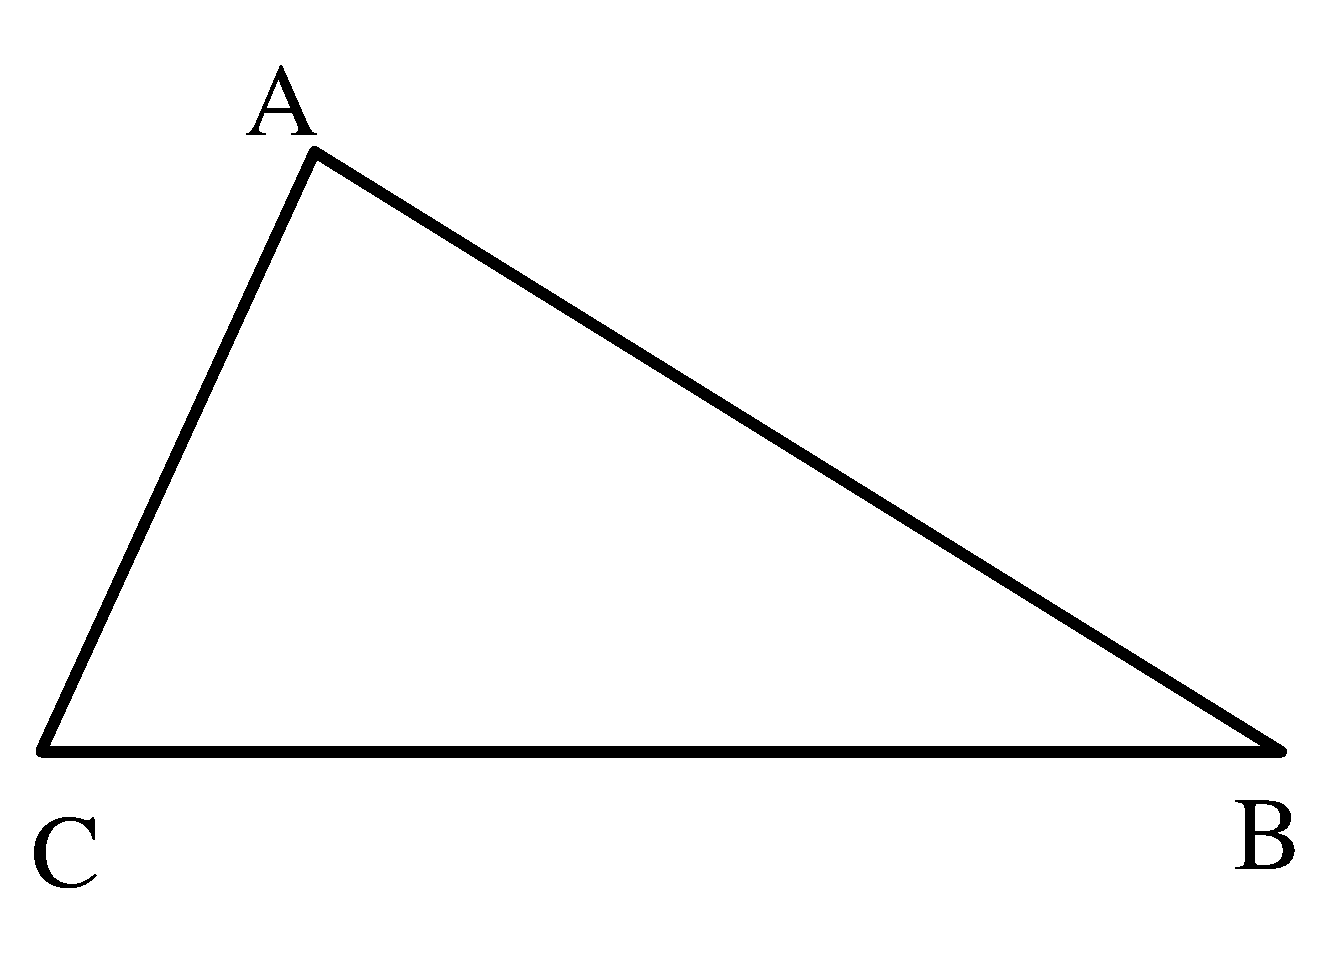
\includegraphics[keepaspectratio, width=3.0cm,height=2.4cm,clip]{eikaku_C.pdf}

                    (A) 鋭角三角形
                \end{center}
            \end{minipage}
            \begin{minipage}{0.5\hsize}
                \begin{center}
                    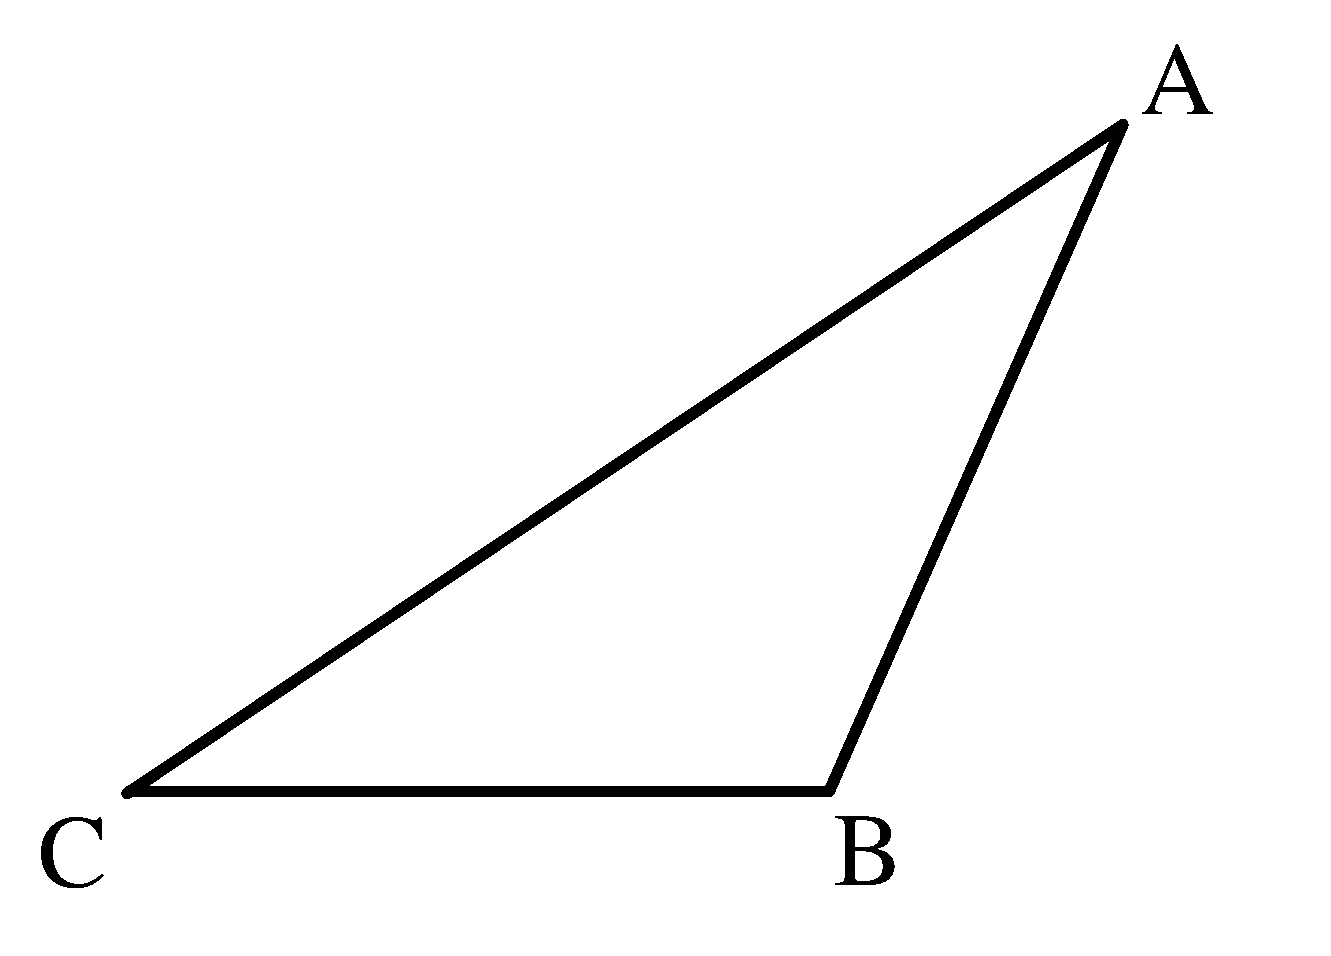
\includegraphics[keepaspectratio, width=3.0cm,height=2.4cm,clip]{donkaku_S.pdf}

                    (B) 鈍角三角形
                \end{center}
            \end{minipage}
        \end{tabular}
        \label{fig:sankakukei_no_katati}
        \caption{三角形の種類}
    \end{figure}

    ここで確認したいのは,$\sin$ 関数と $\cos$ 関数である.
    図の三角形(鋭角,鈍角のどちらでもよい)で,三角形の頂点Aから,辺BCもしくはその延長に
    対して垂線を引く.垂線の足
        \footnote{
            垂線の足:頂点Aから辺BCの延長の交点のこと.
        }
    を $H$ とする.$\angle \mathrm{ABC}$ の角度を $\theta$ と表す.
    \begin{figure}[hbt]
        \begin{tabular}{cc}
            \begin{minipage}{0.5\hsize}
            \begin{center}
                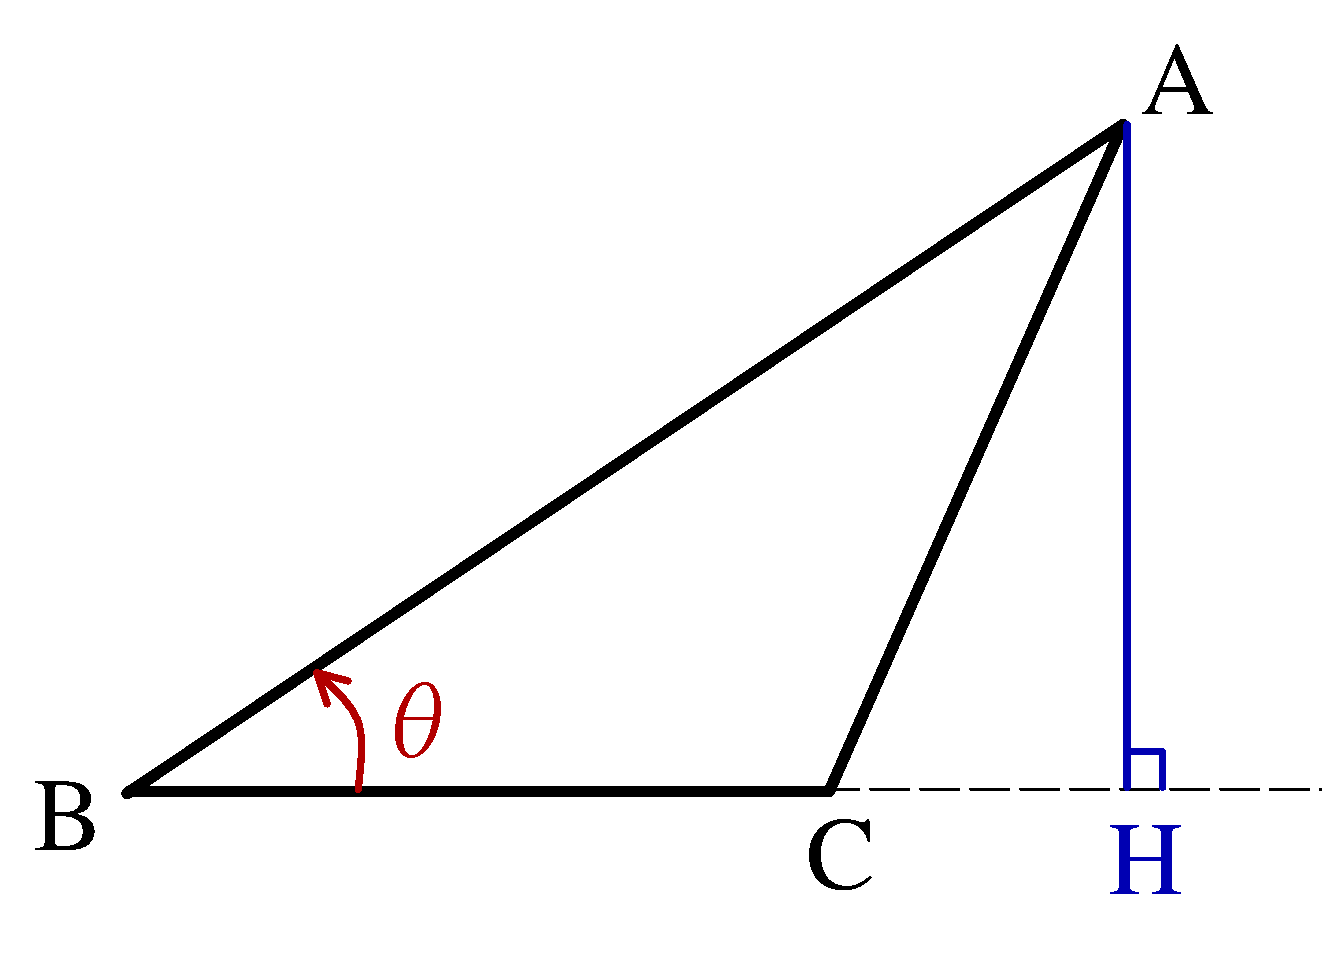
\includegraphics[keepaspectratio, width=3.5cm,height=2.8cm,clip]{function_sin_1.pdf}

                (A)
            \end{center}
            \end{minipage}
            \begin{minipage}{0.5\hsize}
            \begin{center}
                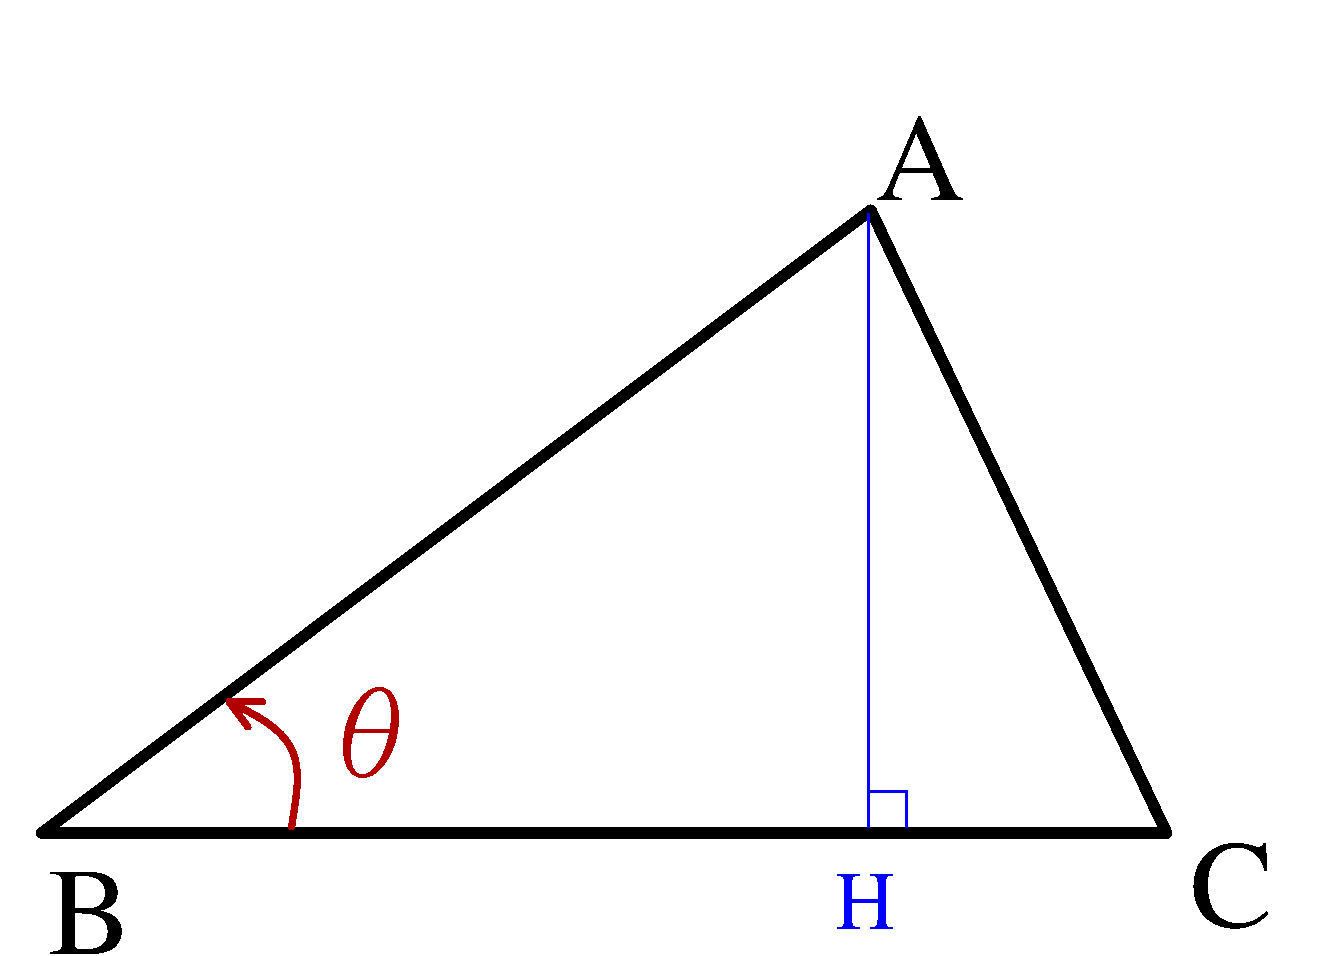
\includegraphics[keepaspectratio, width=3.5cm,height=2.8cm,clip]{function_sin_2.pdf}

                (B)
            \end{center}
            \end{minipage}
        \end{tabular}
        \caption{垂線の引き方}
        \label{fig:suisen_no_hikikata}
    \end{figure}

    これから大事なるのが,垂線AHとBHである.
    つまり,直角三角形を考えることになる.
    三角比には一般の三角形で成り立つような,
    「正弦定理」や「余弦定理」などがあるが,これらはここでは
    考えず,必要になった時に確認するという形にしたい.
    とりあえずは直角三角形を考える.

    ということで,図を以下のように書き直そう.
        \begin{figure}[hbt]
            \begin{center}
                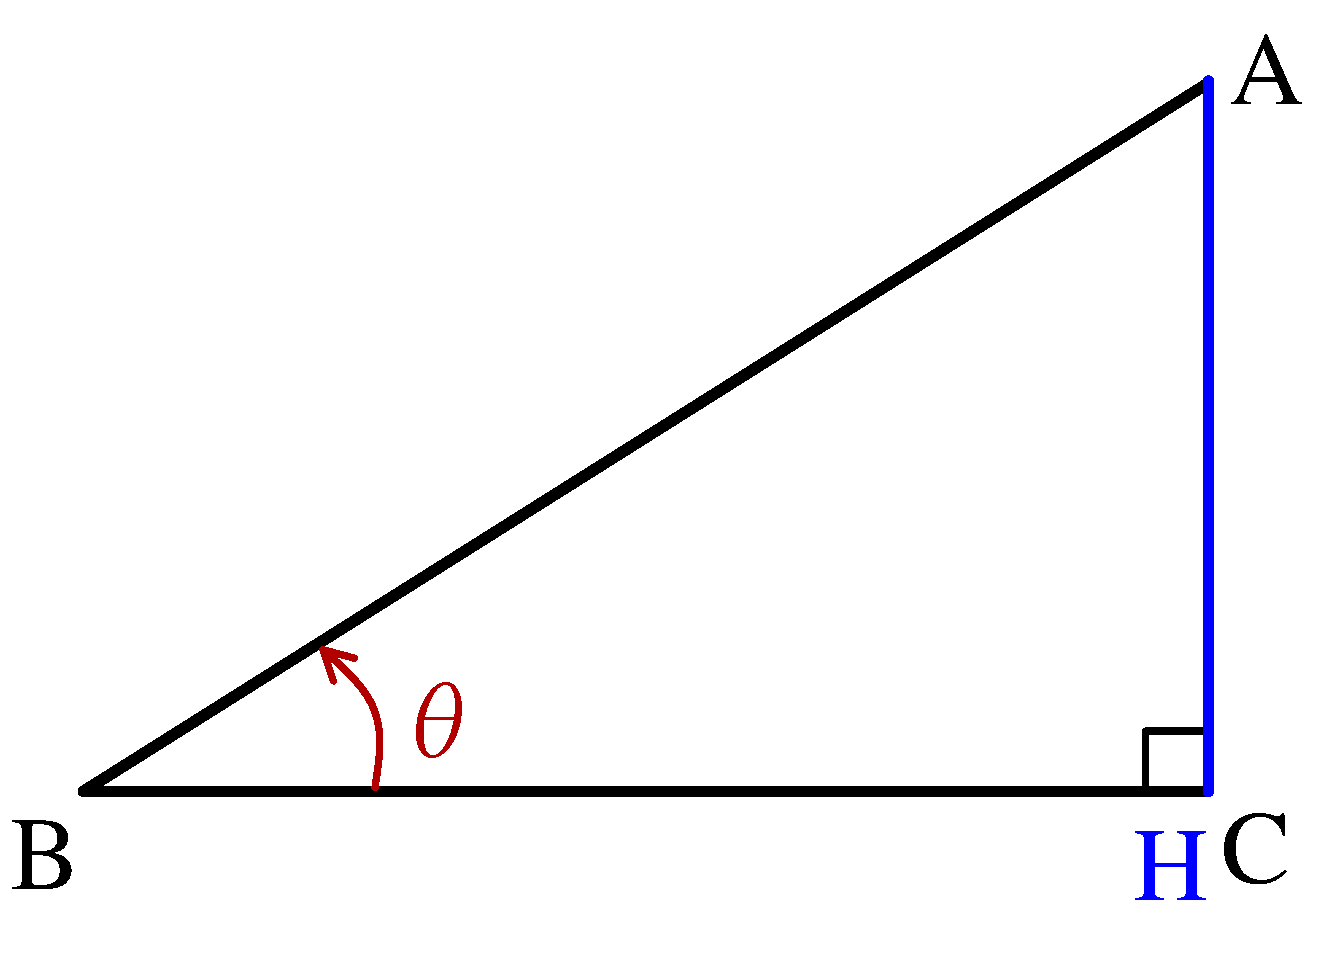
\includegraphics[keepaspectratio, width=3.5cm,height=2.8cm,clip]{sincos111.pdf}
                \caption{直角三角形の図}
                \label{fig:sincos111}
            \end{center}
        \end{figure}

    直角三角形は,辺ABの長さ $\|\mathrm{AB}\|$ と角度 $\theta$ で,その形を特定できる.
        \footnote{
            言い換えると,$\|\mathrm{AB}\|$ と $\theta$ の2つが特定されると,
            三角形の形とその大きさがきまる,ということ.
        }
    つまり,$\|\mathrm{AB}\|$ と $\theta$ がそれぞれ
    1つずつ定まれば,垂線AHの長さ $\|\mathrm{AH}\|$ が1つに定まるという関係がある.
    従って,$\|\mathrm{AH}\|$ は,$\|\mathrm{AB}\|$ と $\theta$ の関数であり,
        \begin{equation*}
            \|\mathrm{AH}\| = \|\mathrm{AB}\|\sin \theta
        \end{equation*}
    と表現する.辺ABが,基準となる水平な線よりも角度 $\theta$ だけ傾いている
    ときの,縦方向の長さが $\|\mathrm{AH}\|$ なのである.
    \begin{figure}[hbt]
        \begin{tabular}{cc}
            \begin{minipage}{0.5\hsize}
            \begin{center}
                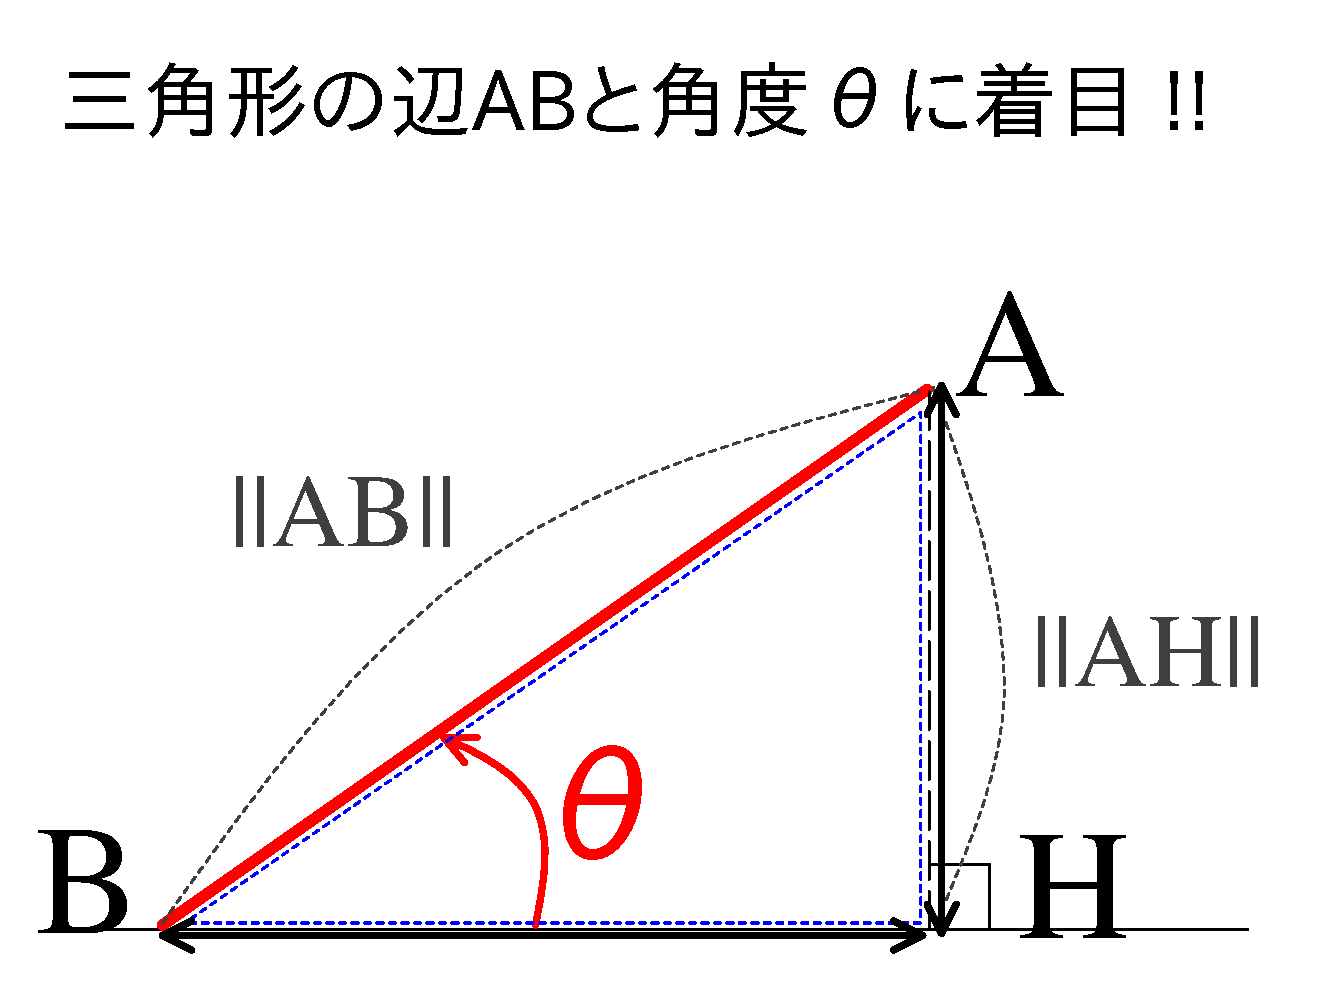
\includegraphics[keepaspectratio, width=3.5cm,height=2.8cm,clip]{sankakuhi-ABH.pdf}

                (A)
            \end{center}
            \end{minipage}
            \begin{minipage}{0.5\hsize}
            \begin{center}
                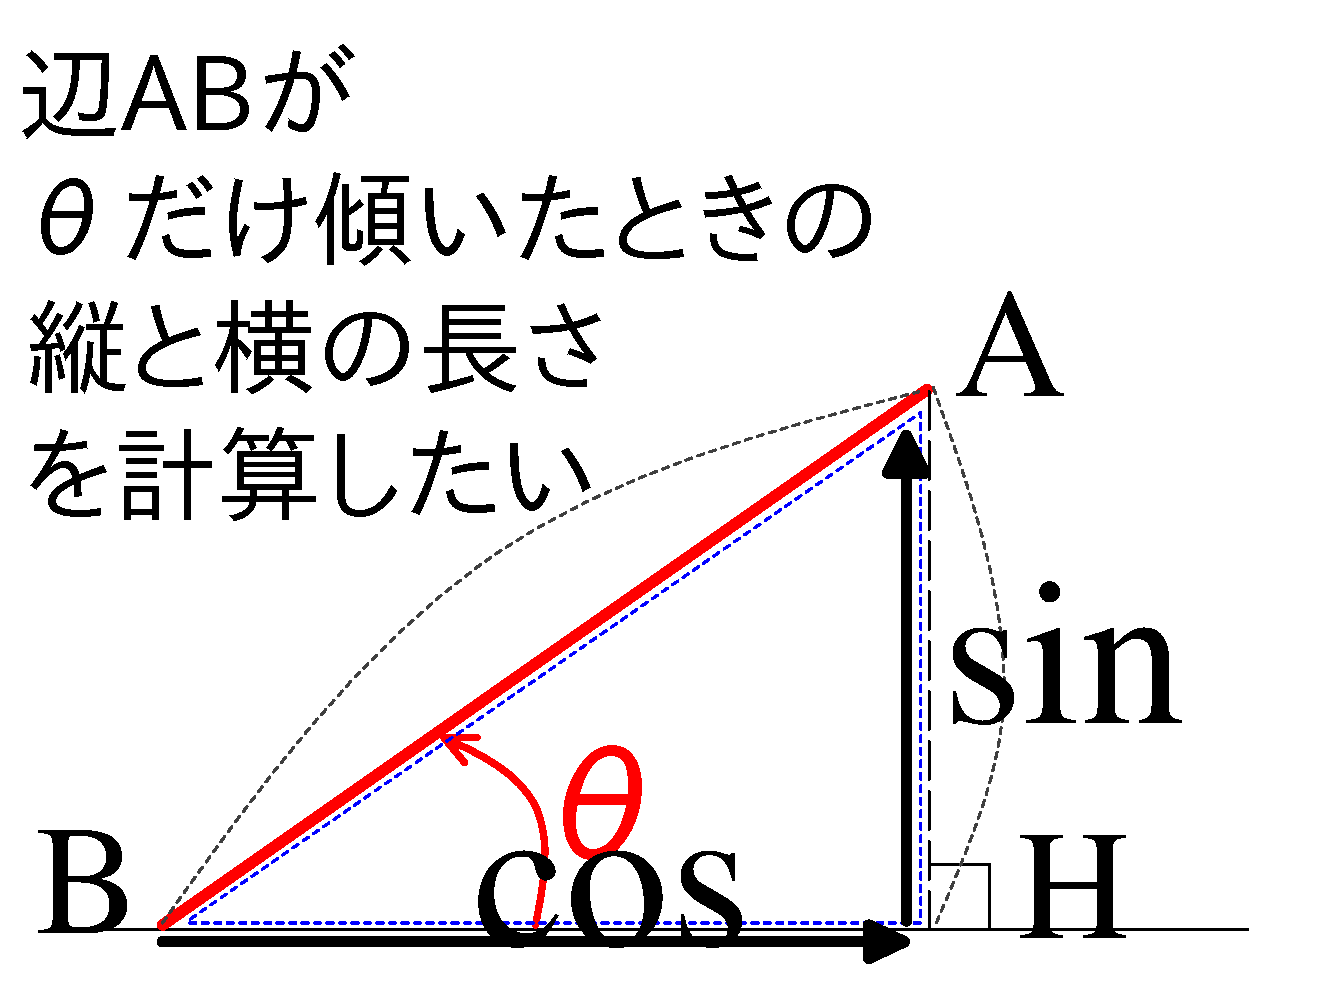
\includegraphics[keepaspectratio, width=3.5cm,height=2.8cm,clip]{sankakuhi-ABH-2.pdf}

                (B)
            \end{center}
            \end{minipage}
        \end{tabular}
        \caption{三角形の見方を変えよう}
        \label{fig:sankakukei-no-mikata}
    \end{figure}

    もう一方の辺BHの長さ $\|\mathrm{BH}\|$ も,$\|\mathrm{AB}\|$ と $\theta$ の関数である.
        \begin{equation*}
            \|\mathrm{BH}\| = \|\mathrm{AB}\|\cos \theta
        \end{equation*}
    と表現する.

    要するに,辺ABが $\theta$ だけ傾いている直角三角形の,
    縦の長さ($\|\mathrm{AH}\|$)が知りたい場合,$\|\mathrm{AB}\|$ に $\sin \theta$ を
    かけて,
        \begin{equation*}
            \|\mathrm{AH}\| = \|\mathrm{AB}\| \sin \theta
        \end{equation*}
    と計算できるということだ.横の長さ($\|\mathrm{BH}\|$)を知りたければ,$\cos \theta$ をかければよく,
        \begin{equation*}
            \|\mathrm{BH}\| = \|\mathrm{AB}\| \sin \theta
        \end{equation*}
    と計算される.$\sin \theta$ と $\cos \theta$ の値は,すでに先人が計算していて,
    今では,三角関数の表として,簡単に参照できるし,$\|\mathrm{AB}\|$ もわかる.
    つまり,三角関数を使うことで,辺ABとその傾射ている角度 $\theta$ から,
    縦と横の長さを計算で出すことができるのだ.

    さらに,$\sin \theta$ と $\cos \theta$ を使うと,
    辺ABの傾きを表現できる.一次関数,
    つまり直線の式
    では,$y=ax+b$ の $a$ が
    直線 $y$ の傾きを表している.
    傾きとは,
        \begin{equation*}
            a=\frac{(y\mbox{の増加量})}{(x\mbox{の増加量})}
        \end{equation*}
    で定義される量であった.この式の分母に $\|\mathrm{AB}\|\cos\theta$を,
    分子に $\|\mathrm{AB}\|\sin\theta$ を入れると,
        \begin{equation*}
            \frac{\sin\theta}{\cos\theta}
        \end{equation*}
    である.($\|\mathrm{AB}\|$ は約分される.)
    これは,辺ABの傾きにほかならない.これを,$\tan$ という関数記号を
    導入し,
        \begin{equation*}
            \tan\theta =\frac{\sin\theta}{\cos\theta}
        \end{equation*}
    と表現する.三角比には他にもいろいろな公式があるが,ここでは省略する.
    三角比は三角関数の特殊($0^{\circ}< \theta <180^{\circ}$)な例である.
    従って,三角比の公式は,三角関数でも成り立つ.三角関数を説明した後,
    そのうちの重要な公式を確認しよう.

    では次に,三角関数にとりかかろう.

\subsubsection{三角関数の定義}
    三角関数の定義する
        \footnote{
            この定義は,図形を用いてなされるので,
            かなり直観的で,何か受け入れがたい
            のだが,とりあえず便宜上の定義として
            考えてもらいたい.しかし,この定義は
            完全に間違っているわけではない.
            図形的に定義されるから,そこに直観が入り,
            論理が崩れてしまうという恐れがあるだけである.
            このノートでは,この図形的定義で十分である.
        }.
    図\ref{fig:sankakukansu1}を参照してほしい.
        \begin{figure}[hbt]
            \begin{center}
                \includegraphicsdefault{sankakukansu1.pdf}
                \caption{三角関数}
                \label{fig:sankakukansu1}
            \end{center}
        \end{figure}

    図を見るときに,半径 $r$ の円上を回転
    しているイメージしてほしい.この回転により,$\theta$ がいろいろな値
    に変化している様子が想像できればよい.${0\,}^{\circ} < \theta < {360\,}^{\circ}$ に
    \textbf{限らず},何回転でもできる.また,右回転(図\ref{fig:sankakukansu1}の矢印の向き)を
    正方向の回転として,その逆回転の負方向の回転も可能である.負の回転の場合,$\theta$ の取りうる
    値は負になる.この回転する半径のことを,\textbf{動径} とよぶ.\\

        \begin{itembox}[l]{三角関数の定義}
            図\ref{fig:sankakukansu1}において,三角関数 $\sin\theta$,
            $\cos\theta$,$\tan\theta$ を次で定義する.
                \begin{align}
                    \sin\theta := \frac{y}{r}\\ \notag \\
                    \cos\theta := \frac{x}{r}\\ \notag \\
                    \tan\theta := \frac{y}{x}
                \end{align}
        \end{itembox}\\
    $r$ は円の半径である.この定義では,もちろん $r  \neq  0$ と仮定している.

\subsubsection{三角関数の図形的イメージ}
    三角関数の定義式を見ても,最初はイメージしにくいここと思う.
    だから,ここで,三角関数の図形的イメージを押さえておこう.

    \begin{mysmallsec}{$\cos$ 関数のイメージ}
        最初に,$\cos$ 関数のイメージを考える.$\cos$ 関数の定義式は
            \begin{equation*}
                \cos \theta = \frac{x}{r}
            \end{equation*}
        である.但し,右辺は直交座標による.$r$ は円の半径であるから,
        定数として見てよい.例えば,$r=1$ の場合を考えてみよう.$r=1$ の
        場合,定義式により
            \begin{equation*}
                \cos \theta = x
            \end{equation*}
        となる.これは何を表しているか.式の示す通りである.
        $\cos \theta$ は $x$ の座標値に等しい.三角形で考えれば,
        半径 $r$ を斜辺とみなしたときの,$x$ 座標に等しいのである.


        半径が1でない場合はどうだろうか.その場合,定義式から,
            \begin{equation*}
                r \cos \theta = x
            \end{equation*}
        である.単に半径が1の場合の $r$ 倍になったにすぎない.


        これは,半径の $x$ 方向だけを考えたい場合に便利な道具となる.
        動径はいろいろな角度に運動するだろうが,その方向全てではなく,
        $x$ 軸方向のみを知りたい場合,その時の動径の角度を $\theta$ と
        して,$\cos \theta$ をかければよいのだ.


        長さ $r$ をもつ動径が,角度 $\theta$ の位置にあるとき,その時の
        $x$ 座標は $x = r \cos \theta$ で計算できる.半径 $r$ に $\cos \theta$ を
        かけると $x$ 座標が分かるのである.

        これはまた,\textbf{動径の $x$ 方向の長さを示している}とみても同じことである.
    \end{mysmallsec}


    \begin{mysmallsec}{$\sin$ 関数のイメージ}
        $\sin$ 関数も,$\cos$ 関数と同じように考えられる.
        $\sin$ 関数の定義は
            \begin{equation*}
                \sin \theta = \frac{y}{r}
            \end{equation*}
        である.
        半径 $r = 1$ の場合,それは動径の $y$ 座標を示す.
        $r\neq1$ の場合は,
            \begin{equation*}
                r \sin \theta = y
            \end{equation*}
        である.これは動径の $y$ 座標に他ならない.
        動径の $x$ 座標を知りたい場合は,半径に $\cos \theta$ を
        かければよいのと同様に,動径の $y$ 座標を知りたい場合は,
        $\sin \theta$ を半径 $r$ にかければよい.

        長さ $r$ をもつ動径が,角度 $\theta$ の位置にあるとき,その時の
        $y$ 座標は $y = r \sin \theta$ で計算できる.半径 $r$ に $\sin \theta$ を
        かけると $y$ 座標が分かるのである.

        これはまた,\textbf{動径の $y$ 方向の長さを示している}とみても同じことである.
    \end{mysmallsec}


    \begin{mysmallsec}{$\tan$ 関数のイメージ}
        では,$\tan$ 関数は同イメージされるのだろう.
        $\tan$ 関数の定義は
            \begin{equation*}
                \tan \theta = \frac{y}{x}
            \end{equation*}
        である.
        定義そのものを見れば,答えは意外に簡単だ.
        動径の傾きを表しているのである.これは定義式から明らかだ.動径の
        一端は常に座標のある一点から動かない.今の場合は,
        考えやすいように,座標原点に一端を固定している.だから,
            \begin{equation*}
                \frac{y}{x} = \frac{y-0}{x-0}
            \end{equation*}
        と見ることができる.動径の回転中心が座標原点ではなく,
        $(\,x_{0},\,y_{0}\,)$ の場合は
            \begin{equation*}
                \frac{y-y_{0}}{x-x_{0}}
            \end{equation*}
        である.どちらの場合も,
            \begin{equation*}
                \frac{y\mbox{の増加量}}{x\mbox{の増加量}}
            \end{equation*}
        と見ることができる.

        \textbf{$\tan$ は,動径を一次関数と見立てた時の,変化の割合を示す量}と
        見ることができる.
    \end{mysmallsec}

\subsubsection{三角関数の性質}
    三角関数には公式がいろいろとある.ここでいくつかを
    確認しておこう.

    まず,三平方の定理から,\\

        \begin{itembox}[l]{三角関数の公式}
            \begin{align}
                \sin^{2} \theta  +  \cos^{2} \theta  =  1
            \end{align}
        \end{itembox}\\
    が成立する.

    \begin{mysmallsec}{説明}
        簡単に説明する.直交座標において,
            \begin{equation*}
                x^{2}  +  y^{2}  =  r^{2}
            \end{equation*}
        が成立する.さて,この $x$,$y$ は三角関数の定義から,
            \begin{equation*}
                x  =   r \cos \theta \quad, \quad y  =  r \sin \theta
            \end{equation*}
        である.つまり,
            \begin{align*}
                x^{2}  +  y^{2}  &=  r^{2} \\
                (r \cos \theta)^{2}  +  (r \sin \theta)^{2}  &=  r^{2} \\
                r^{2} \cos^{2} \theta  +  r^{2} \sin^{2} \theta  &=  r^{2}.
            \end{align*}
        $r\neq0$ だから $r^{2} \neq 0$ であり,$r^{2}$ で割ると,
            \begin{equation*}
                \sin^{2} \theta  +  \cos^{2} \theta  =  1
            \end{equation*}
        が導かれる.
    \end{mysmallsec}

